\subsection{Nos machines}
Dans le but d'étudier différents problèmes liés à la programmation par tâche, nous avons sélectionné deux machines avec des architectures différentes.

\subsubsection{Rostand}
Rostand est une grappe de serveurs appartenant à la compagnie Total S.A..
%
Elle est composée de 640 noeuds de calcul interconnectés avec un réseau Infiniband.
%
Chaque noeud est lui-même composé de 2 bancs NUMA avec un processeur Intel Xeon X5660 et 24~GO de mémoire par banc NUMA (Fig.~\ref{fig:rostand}).
%
Les processeurs ont 6 coeurs, soit un total de 12 coeurs par noeud de calcul et 7680 coeurs pour l'ensemble de la grappe.

%   (-_-)   %
\begin{figure}[!ht]
        \centering
        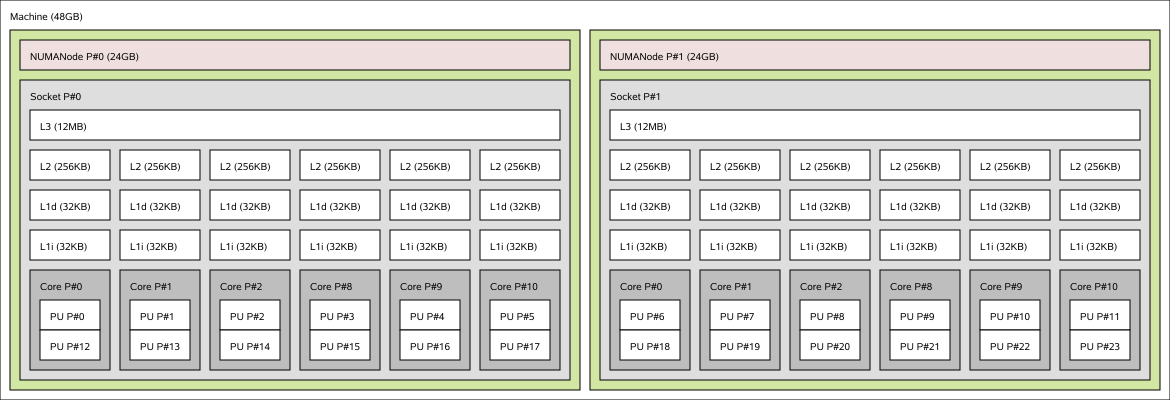
\includegraphics[width=\textwidth]{rostand_lstopo}
        \caption{Topologie d'un noeud de calcul de Rostand. Le schéma a été obtenu avec le logiciel hwloc.}
        \label{fig:rostand}
\end{figure}

Avec cette machine, nous allons pouvoir tester deux paradigmes de programmation parallèle.
%
Dans un premier temps nous allons faire du parallélisme intra-noeud puis nous verrons le parallélisme inter-noeud.

\subsubsection{Manumanu}
Manumanu est une machine Altix UV100, cet ordinateur est composé de 20 bancs NUMA.
%
Chaque banc NUMA est composé d'un processeur Intel Xeon E7-8837 ainsi que de 32~GO de mémoire.
%
Les processeurs ont chacun 8 coeurs de calcul, pour un total de 160 coeurs et 640~GO de mémoire partagée.
%
Cette machine est vraiment intéressante pour évaluer les effets NUMA.

%   (-_-)   %
\begin{figure}[!ht]
     \begin{center}
        \subfigure[Matrice des distances entre chaque banc NUMA. Résultat obtenu avec la commande ``numactl --hardware''.]{%
          \label{fig:manumanu_distance}
          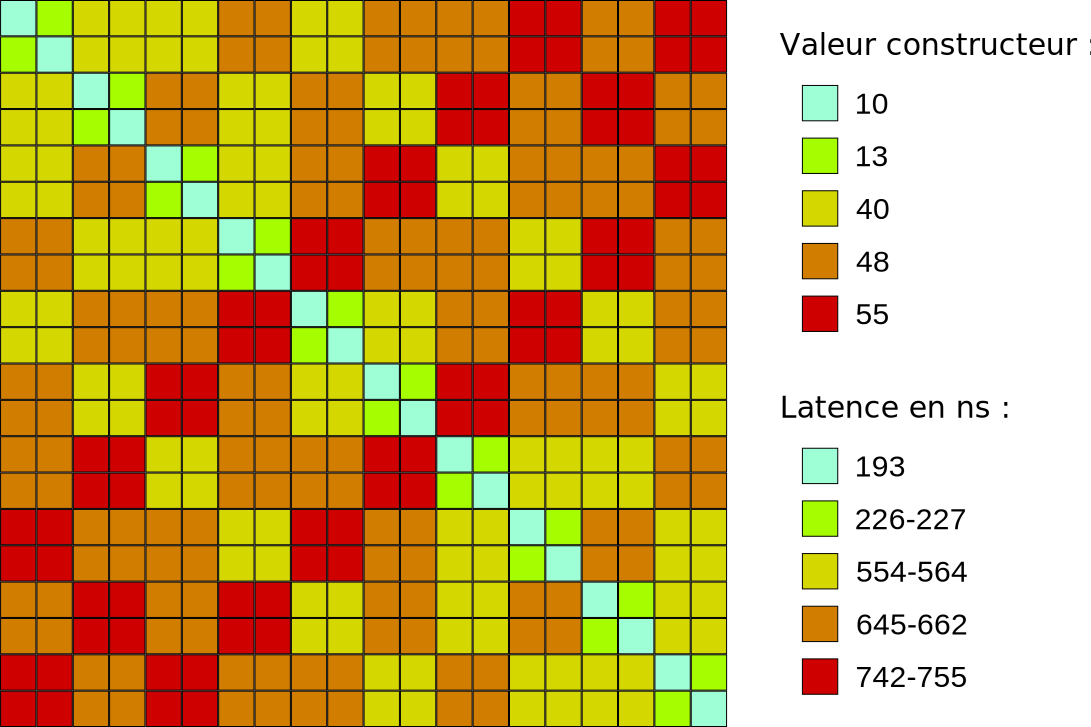
\includegraphics[width=0.49\textwidth]{manumanu_distance}
        }%
        \subfigure[Topologie de Manumanu déduite de la matrice des distances. Chaque noeud représente un ensemble de deux bancs NUMA.]{%
          \label{fig:manumanu_topo}
          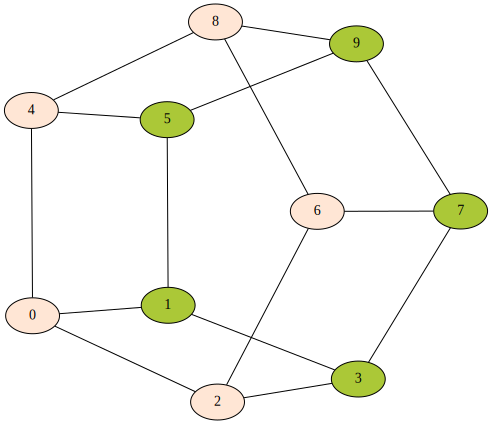
\includegraphics[width=0.49\textwidth]{manumanu_topologie}
        }%
    \end{center}
    \caption{Architecture de Manumanu.}
    \label{fig:manumanu}
\end{figure}

\`{A} partir de la matrice des distances (Fig.~\ref{fig:manumanu_distances}), nous pouvons déduire la topologie de la machine.
%
Les bancs NUMA sont regroupés deux par deux et chaque groupe est connecté à trois autres groupes.
%
Ce regroupement permet de limiter la distance maximal entre deux banc NUMA, il y aura au maximum 3 sauts.
